\documentclass[conference]{IEEEtran}
\usepackage[top=2.5 cm, bottom=2.5 cm, left=2.0 cm, right=2.0 cm]{geometry}
\geometry{letterpaper}
\usepackage[parfill]{parskip}
\usepackage{graphicx}
\usepackage{amsmath}
\usepackage{amssymb}
\usepackage{comment}
\usepackage{epstopdf}
\usepackage{subfigure}
\usepackage{extarrows}
\usepackage{minted}
\usemintedstyle{vs}

\DeclareGraphicsRule{.tif}{png}{.png}{`convert #1 `dirname #1`/`basename #1 .tif`.png}



\title{Realtime 6DOF SLAM for a Quadrotor Helicopter}

\author{\IEEEauthorblockN{Stephen Chaves}
  \and
  \IEEEauthorblockN{Schuyler Cohen}
  \and
  \IEEEauthorblockN{Patrick O'Keefe}
  \and
  \IEEEauthorblockN{Paul Ozog}}

% \IEEEauthorblockA{School of Electrical and\\Computer Engineering\\
% Georgia Institute of Technology\\
% Atlanta, Georgia 30332--0250\\
% Email: http://www.michaelshell.org/contact.html}



\begin{document}
\maketitle



\begin{abstract}
  Lorem ipsum dolor sit amet, consectetur adipisicing elit, sed do eiusmod tempor incididunt
  ut labore et dolore magna aliqua. Ut enim ad minim veniam, quis nostrud exercitation
  ullamco laboris nisi ut aliquip ex ea commodo consequat. Duis aute irure dolor in
  reprehenderit in voluptate velit esse cillum dolore eu fugiat nulla pariatur. Excepteur
  sint occaecat cupidatat non proident, sunt in culpa qui officia deserunt mollit anim id
  est laborum.
\end{abstract}






\section{Introduction}
\label{sec:introduction}

Lorem ipsum dolor sit amet, consectetur adipisicing elit, sed do eiusmod tempor incididunt
ut labore et dolore magna aliqua. Ut enim ad minim veniam, quis nostrud exercitation
ullamco laboris nisi ut aliquip ex ea commodo consequat. Duis aute irure dolor in
reprehenderit in voluptate velit esse cillum dolore eu fugiat nulla pariatur. Excepteur
sint occaecat cupidatat non proident, sunt in culpa qui officia deserunt mollit anim id
est laborum.






\section{Parrot AR.Drone}
\label{sec:parrotar.drone}

Lorem ipsum dolor sit amet, consectetur adipisicing elit, sed do eiusmod tempor incididunt
ut labore et dolore magna aliqua. Ut enim ad minim veniam, quis nostrud exercitation
ullamco laboris nisi ut aliquip ex ea commodo consequat. Duis aute irure dolor in
reprehenderit in voluptate velit esse cillum dolore eu fugiat nulla pariatur. Excepteur
sint occaecat cupidatat non proident, sunt in culpa qui officia deserunt mollit anim id
est laborum.






\section{Incremental Smoothing and Mapping}
\label{sec:incrementalsmoothingandmapping}

I guess we need to cite something for this to compile. \cite{Kaess08tro}

Lorem ipsum dolor sit amet, consectetur adipisicing elit, sed do eiusmod tempor incididunt
ut labore et dolore magna aliqua. Ut enim ad minim veniam, quis nostrud exercitation
ullamco laboris nisi ut aliquip ex ea commodo consequat. Duis aute irure dolor in
reprehenderit in voluptate velit esse cillum dolore eu fugiat nulla pariatur. Excepteur
sint occaecat cupidatat non proident, sunt in culpa qui officia deserunt mollit anim id
est laborum.


\subsection*{Givens Rotations}
\label{sub:givensrotations}

Lorem ipsum dolor sit amet, consectetur adipisicing elit, sed do eiusmod tempor incididunt
ut labore et dolore magna aliqua. Ut enim ad minim veniam, quis nostrud exercitation
ullamco laboris nisi ut aliquip ex ea commodo consequat. Duis aute irure dolor in
reprehenderit in voluptate velit esse cillum dolore eu fugiat nulla pariatur. Excepteur
sint occaecat cupidatat non proident, sunt in culpa qui officia deserunt mollit anim id
est laborum.


\subsection*{Variable Reordering}
\label{sub:variablereordering}

Lorem ipsum dolor sit amet, consectetur adipisicing elit, sed do eiusmod tempor incididunt
ut labore et dolore magna aliqua. Ut enim ad minim veniam, quis nostrud exercitation
ullamco laboris nisi ut aliquip ex ea commodo consequat. Duis aute irure dolor in
reprehenderit in voluptate velit esse cillum dolore eu fugiat nulla pariatur. Excepteur
sint occaecat cupidatat non proident, sunt in culpa qui officia deserunt mollit anim id
est laborum.


\begin{figure}[!h]
  \begin{center}
    \subfigure[] {
    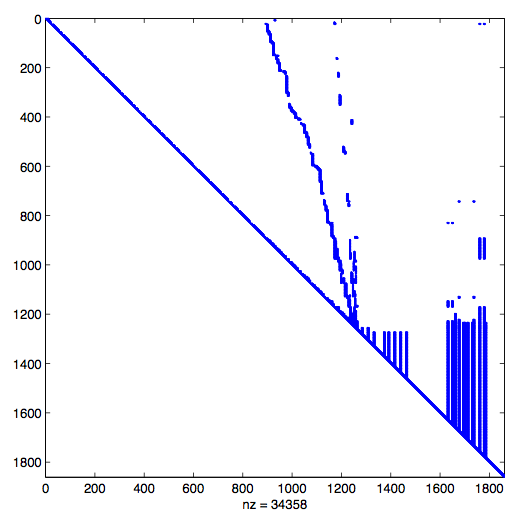
\includegraphics[width=2.5in]{images/reorder32}
    \label{fig:images/reorderResult32Resized}}
    \subfigure[] {
    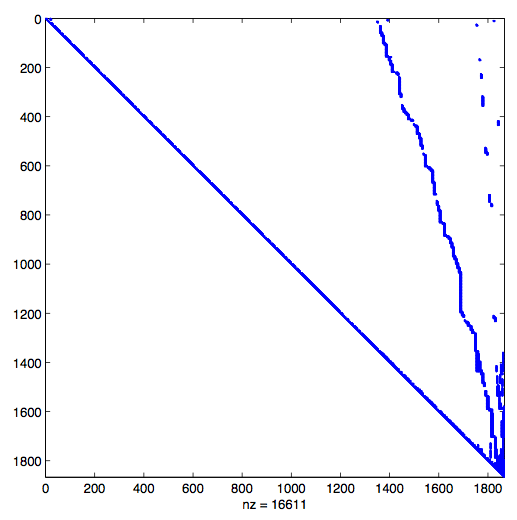
\includegraphics[width=2.5in]{images/reorder33}
    \label{fig:images/reorderResult33Resized}}
    \caption{asdfasdf}
    \label{fig:reorder}
  \end{center}
\end{figure}









\section{AprilTag Covariance Projection}
\label{sec:tagcovarianceprojection}

Lorem ipsum dolor sit amet, consectetur adipisicing elit, sed do eiusmod tempor incididunt
ut labore et dolore magna aliqua. Ut enim ad minim veniam, quis nostrud exercitation
ullamco laboris nisi ut aliquip ex ea commodo consequat. Duis aute irure dolor in
reprehenderit in voluptate velit esse cillum dolore eu fugiat nulla pariatur. Excepteur
sint occaecat cupidatat non proident, sunt in culpa qui officia deserunt mollit anim id
est laborum.









\section{Experiments}
\label{sec:experiments}

Lorem ipsum dolor sit amet, consectetur adipisicing elit, sed do eiusmod tempor incididunt
ut labore et dolore magna aliqua. Ut enim ad minim veniam, quis nostrud exercitation
ullamco laboris nisi ut aliquip ex ea commodo consequat. Duis aute irure dolor in
reprehenderit in voluptate velit esse cillum dolore eu fugiat nulla pariatur. Excepteur
sint occaecat cupidatat non proident, sunt in culpa qui officia deserunt mollit anim id
est laborum.


\subsection*{Simulation}
\label{sub:simulation}

Lorem ipsum dolor sit amet, consectetur adipisicing elit, sed do eiusmod tempor incididunt
ut labore et dolore magna aliqua. Ut enim ad minim veniam, quis nostrud exercitation
ullamco laboris nisi ut aliquip ex ea commodo consequat. Duis aute irure dolor in
reprehenderit in voluptate velit esse cillum dolore eu fugiat nulla pariatur. Excepteur
sint occaecat cupidatat non proident, sunt in culpa qui officia deserunt mollit anim id
est laborum.

\begin{figure}[!t]
  \centering
  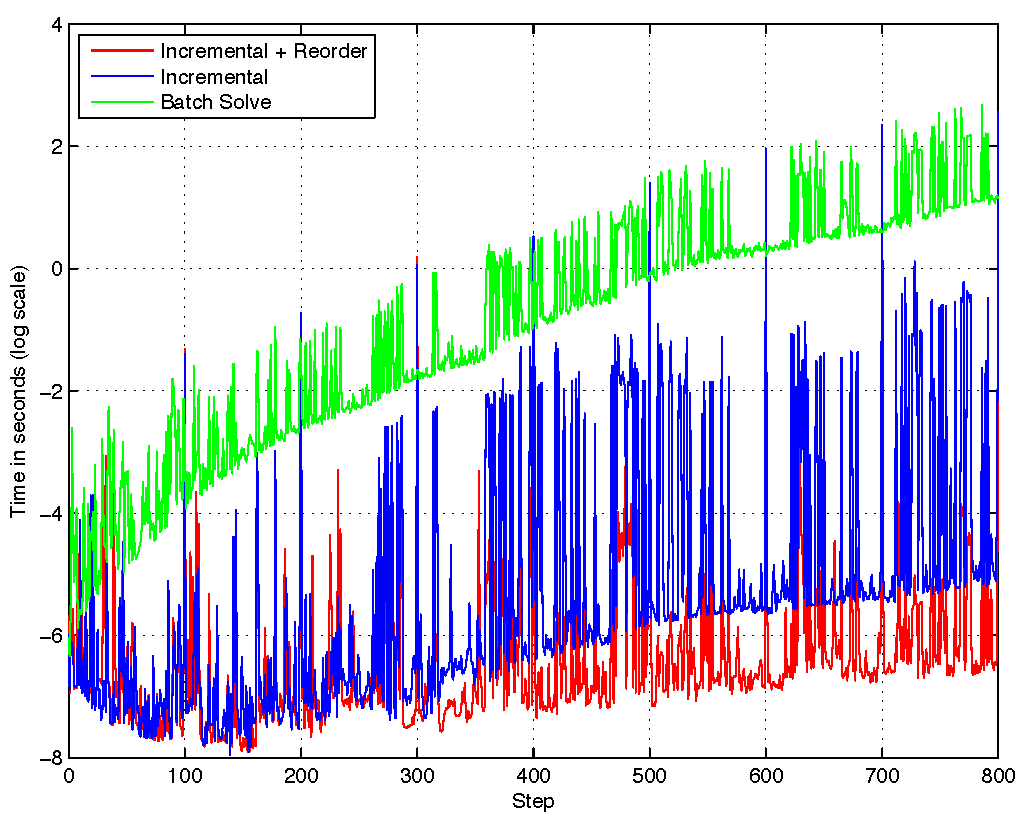
\includegraphics[width=2.5in]{images/stepTimeResults}
  \caption{The time per step for different SLAM solve methods.}
  \label{fig:stepTime}
\end{figure}


\subsection*{Quadrotor}
\label{sub:quadrotor}

Lorem ipsum dolor sit amet, consectetur adipisicing elit, sed do eiusmod tempor incididunt
ut labore et dolore magna aliqua. Ut enim ad minim veniam, quis nostrud exercitation
ullamco laboris nisi ut aliquip ex ea commodo consequat. Duis aute irure dolor in
reprehenderit in voluptate velit esse cillum dolore eu fugiat nulla pariatur. Excepteur
sint occaecat cupidatat non proident, sunt in culpa qui officia deserunt mollit anim id
est laborum.










\section{Conclusion}
\label{sec:conclusion}


Lorem ipsum dolor sit amet, consectetur adipisicing elit, sed do eiusmod tempor incididunt
ut labore et dolore magna aliqua. Ut enim ad minim veniam, quis nostrud exercitation
ullamco laboris nisi ut aliquip ex ea commodo consequat. Duis aute irure dolor in
reprehenderit in voluptate velit esse cillum dolore eu fugiat nulla pariatur. Excepteur
sint occaecat cupidatat non proident, sunt in culpa qui officia deserunt mollit anim id
est laborum.



\section*{Acknowledgment}

The authors would like to thank Sprite, the number 7, and Emacs.



\bibliographystyle{IEEEtran}
% argument is your BibTeX string definitions and bibliography database(s)
\bibliography{IEEEabrv,references}


\end{document}



% An example of a floating table. Note that, for IEEE style tables, the
% \caption command should come BEFORE the table. Table text will default to
% \footnotesize as IEEE normally uses this smaller font for tables.
% The \label must come after \caption as always.
%
% \begin{table}[!t]
%%   increase table row spacing, adjust to taste
%   \renewcommand{\arraystretch}{1.3}
%   if using array.sty, it might be a good idea to tweak the value of
%   \extrarowheight as needed to properly center the text within the cells
%   \caption{An Example of a Table}
%   \label{table_example}
%   \centering
%%   Some packages, such as MDW tools, offer better commands for making tables
%%   than the plain LaTeX2e tabular which is used here.
%   \begin{tabular}{|c||c|}
%     \hline
%     One & Two\\
%     \hline
%     Three & Four\\
%     \hline
%   \end{tabular}
% \end{table}
